%\section{Graph isomorphism}

%Weisfeiler-Lehman Test

\section{Distributions}

\subsection{power-law}
Power-law distributions characterize many social and biological systems. Power-law distributions are also easy to generate. 

the distributions: basic definitions and properties

The nonnegative random variable X is said to have a power law distribution if 
\begin{equation}
Pr[X>x] \sim c x ^{-\alpha}
\end{equation}

for constants $c>0$ and $\alpha >0$. In power-law distribution asymptotically the tails fall according to power $\alpha$. Such distribution leads to much havier tails than other common models, as exponential distribution. 

One specific power-law distribution is Pareto distribution which satisfies 

\begin{equation}
	Pr[X>x] = \frac{x}{k} ^{-\alpha}
\end{equation}

for some $\alpha>0$ and $k>0$. The Pareto requires $X>k$. The density function of Pareto distribution is $f(x)=\alpha k^\alpha x^{-\alpha-1}$. For power law distribution $\alpha$ is in the range $0 < \alpha < 2$, in which case X has infinite variance, if alpha <1 X has infinite mean.

if X has power law distribution, then a in log-log plot $Pr(x)$ will behave as straight line. For the specific case of Pareto distribution, the behaviour is exactly linear as $ln (Pr(x)) = -\alpha (lnx -ln k) $. Similarly the density function is also straight line. $ln(f(x)) = (-\alpha - 1) ln (x) + \alpha ln (k) + ln(a)$

\subsection{log-normal}
Many measurments in the nature show a more or less skewed distribution. They are common when mean values are low, variances are large and values can not be negative as example in distribution of minearal resources in the Eart. Such skewed distributions often closely fit to log-normal distribution. 

What is the difference between normal and lognormal variability? A major difference is that effect can be additive or multiplicative, leading to normal or lognormal distribution. Basic principles of additive and multiplicative effects can be easily demonstrated with the help od two dices. Adding the two numbers, which is the principle of the most games, leads to values from 2 to 12 with mean of 7, and simetrical frequency distribution. Multiplying the two numbers, leads to values from 1 to 36 with highly skewed distribution. Although these examples are not normal or lognormal they give us clear difference how different distributions can emerge. 

Log-normal distributions are usually characterized in the term of the log-transformed variable, using as parameters the expected value, or the mean, and the standard deviation. This characerization can be advantageous as by definition log-normal distributions are simetrical at the log level. 

The basic properties of the lognormal distributions

Random variable $X$ if $log(X)$ is normally distributed., if $Y=ln X$ has normal Gaussian distribution.  

Only positive values are possible for the variable and distribution is skewed. Two parameters are needed to specify lognormal distribution. Traditionaly the mean $\mu$ and standard deviation $\sigma$ or the variance of the $\sigma^2$ of $log(X)$ are used. However there are clear advantages of using transformed data, $\mu^{*} = e^{\mu}$, $\sigma^{*}= e ^{\sigma}$. The median of this lognormal distribution is $med(X)=\mu^{*}=e^{\mu}$, since $\mu$ is median of the $log(X)$.

\begin{equation}
f(x) = \frac{1}{x \sigma \sqrt{2\pi}}exp(-\frac{1}{2\sigma^2}(log(x)-\mu)^2)
\end{equation}

The mean is $exp(\mu + \sigma /2)$ and variance is $(exp(\sigma^2)-1)exp(2\mu+\sigma^2)$. 

Estimation: The asymptotically most efficient (maximum likelihood) estimators are 
\begin{equation}
x* = exp (\frac{1}{n}\sum_{i=1}^n log(x_i)) = (\prod_{i=1}^nx_i)^{\frac{1}{n}}
\end{equation}

\begin{equation}
s* = exp([\frac{1}{n-1}\sum[log(\frac{x_i}{x*})]^2]^{\frac{1}{2}})
\end{equation}


The lognormal distribution is skewed with mean $e^{\mu + \frac{1}{2}\sigma^2}$, median $e^\mu$ and mode $e^{\mu - \sigma^2 }$. It has finite mean and variance, in contrast to the power-law distribution.  

Despite it has finite moments, the lognormal distribution can be similar to power-law. If $X$ has a lognormal distribution then loglog plot of density function can apear as straight line for a large portion of a body of distribution. If the variance is large, the distribution may appear linear on log-log plot for several orders of magnitude. The variance of the corresponding normal distribution is large, the distribution may appear linear on a log-log plot. To see this we can check the logarithm of density function. 
If $\sigma$ is large then the quadratic term will be small for large range of x values, so the logarithm of the density function will appear almost linear for large range of values. 
Recall that normal distribution have property that the sum of two independent normal variables is normal variable. It follows that product of two lognormaly distributed random variables also has a lognormal distribution. 

%\section{Scale-free networks}

%The study of scale ivariance has a long tradition. Among the fields where this property was analysed were the theory of critical phenomena, percolations and fractal geometry. One of the first examples considered eas the price fluctuations  of cotton in commodities market (Mandelbort, 1963). The future price can not be obtained with arbitary precision from past series., still this series have some form of regularity. The curves for daily, weakly and montly price fluctuations are statistically similar. The fact that some features are found at different time scales is typical sign of fractal behaviour. Similarly in the case of coastline lenght we find fractal behavior. If we try to measure the total lenght, the real shape is so complicated that we always miss some part. 

%Fractal behaviour might refer to different properties. In some systems scale-free structure is in shape. In this class the fractal shape can be robust, as in the case of branched patterns or electric breakdown. We say robust because these phenomena happen for varaity of external conditions. In the same class we have other systems that are more fragile, in the sense that they arise after precise tuning of some physical quantity. This is in the case of percolations and critical phenomena. Scale-free invariance may be related with dynamics or evolution of the system. The time activity of the system may display self-similar behaviour. The only sign of fractal behaviour is the mathematical form, power-law fluctuations of the time-series. 

%The self-similarity can be present in the way the different parts of a system interact with each other. This is the case with self-similar graphs and the power-law scaling appers in the distribution of topological quantities like the number of interactions per part  of the system. These phenomena are fractals in the topology. 

%\section{Scale-invariance and power laws}

%The mathematical form of self similarity is represented by powe-laws. Whenever the function $y = f(x)$ can be represented as a constant to the power of x. The physical example is elastic force, the gravitational and electrostatic force. In the case of fractals, their geometry can be identified by considering the numbe of boxes $N(\epsilon)$, of linear size $1/\epsilon$. $N(\epsilon) = \epsilon ^{-D}$, where D is called fractal dimension. D can also be defined using mass relation $M = L^ D$.

%Scale invariance is not restrected to geometry, but also appears in dynamical systems. In this case we have power-law distribution for different physical\setsecnumdepth{subsection} quantit\setsecnumdepth{subsection}ies. For example the evolution of some systems (sanspiles, number of species in the ecosystem) proceeds  with series of causally connected events whose size s is distributed as power-law. $P(s) s^{-\tau}$.

%\subsection{plotting a power-law}

%if we plot the data on double logarithmic scale, we should obtain a straight line. $y = x^{\alpha}$, $ln(y) = \alpha ln(x)$. The tail of the distributon is very noisy, and it is general feature of many experiments. To avoid the fluctuations in the tail it is common to use "binning" or cumulative distribution. 

%In this method the noise reduction is done by deviding the $x$ axis into bins, and averaging the data within each bin. As an example we can take the frequency of numbers between numbers $1$ and $10$. Let assume that bin is $10$ units wide, we can represent all data in one point $b$, with $xb$ given by average of the bin extremes and $yb$ given by the avarage value of $ys$. If the bin size is constant for large values of $x$ the density of bins becomes very large as well. 

%In the case of powerlaws it is usufull to use logarithmic binning. For example take the size of the first bin to be 2, and the others are power of 2. $2^1, 2^2...$. A possible choice is to take as yb the average of the values ys in the bin, and as xb the geometrical average of the bin extremes. Bins are equaly spaced on logarithmic scale. The base can be any number larger than 1, for example 1.2. The drawbacks of this procedure are following: this method does not complitly reduce the noise and the choice of the most appropiate bin size must be determined by using trial and error. In general, small and noisy dataset , the behavior in the tail of distribution can be lost if the bins are too wide. Too small bins will not average the present fluctuations

%Using the method of cumulative distribution instead of calculating the probability that certain value x appears in the experiment, we focus on the probability that an outcome is larger than x. 

%For power-law, 
%$P>(x) = \int_{x}^{\inf} P(x^{'})dx^{'}$.
% For power law cumulative distribution is still powerlaw but with modified exponent. $-\alpha+1$. Still, in this method, if exponent is close to one, integral does not behave like powe-law, reather logarithm. The upper limit is a finite value $x_{max}$ and this can change the shape of curve. 

%The cumulative distribution will resemble a power law only as the value of $xmax$ tends to infinity. Otherwise, the deviation from the straight line could make estimating the exponent very difficult.

%\subsection{multiplicative processes}

%While many power laws are originated by some ‘complex’ mechanism, some others have a very simple explanation. By using multiplicative processes we can obtain quite naturally both power laws and log-normal distributions (that can look like power laws) (Goldstein, Morris, and Yen, 2004). We do not enter here into the debate over whether observed data can be best fit by power law or log-normal variables. Here it is enough to note that the mechanism of multiplicative process is probably the most immediate model for fat-tail phenomena in nature since it naturally produces both.

%Many textbooks and scientific papers deal with this topic. Some of them are very beautiful and complete and we suggest them for further reading (e.g. Mitzenmacher 2004; Newman 2005). Suppose you have an evolution process, where for example an organism transforms itself in time. As a general statement, the state S t at time t will be determined by the previous states and by the external conditions. Whenever the state of the system can be written as we have a multiplicative process. In other words, in a multiplicative process, the state of the system at time t is proportional to the state at time t-1. In biology this could represent the fact that the growth of an organism is ruled by its body mass at the previous step. In the case of city growth (Zanette and Manrubia, 1997; Manrubia and Zanette, 1998; Gabaix, 1999) this equation states that the population at a certain time step is proportional to what it was previously. In both cases the proportionality constant is given by the factor t that can change its value at any time step. Turning back to eqn 4.114 we can immediately see that the variable S t is determined by the product of the various tau where tau is between 0 and t This sum of the logarithms of the tau (under very mild conditions) is a variable following a normal distribution (regardless of the distribution of the tau ). This result comes from the application of the ‘central limit theorem’. This theorem states that, in certain very general hypotheses, the sum of identi- cally distributed random variables with finite variance is a new stochastic variable normally distributed. Therefore, if ln(S t ) is normally distributed, the variable S t is log-normally distributed. This very simple mechanism has been rediscovered and explained over and over many times since the definition of log-normal distributions in 1879 (McAlister, 1879). One of the first applications of these ideas traces back at least to the economist Gibrat (1930, 1931) who uses essentially this model under the name of proportionate effect. Using a different terminology, a somewhat similar idea was introduced at the beginning of last century for biological problems (Kapteyn 1903, 1918). With this idea we have two possible outcomes. As explained above we have true log-normal distributions that can easily be confused with power laws. This happens whenever the log-normal distribution is studied in a range of k for which $\sigma >> ln(k)$. On the other hand, a very similar situ- ation also triggers the formation of true power laws as shown in the next subsection. Powerlaws from multiplicative processes.

%\section {Preferential attachment}

%One of the most successful applications of multiplicative processes is given
%by preferential attachment. To date, this is the most successful mechanism adopted in the study of growing networks. Interestingly, the idea that we are going to explain has been independently rediscovered several times in different fields and ages. Precisely for this reason it has also been given several names. For example: Yule Process, Matthew effect, Rich gets richer, Preferential Attachment, Cumulative advantage. In the community there is some agreement (Mitzenmacher, 2004; New- man, 2005) that the first to present this idea has been G. Yule (1925) in order to explain the relative abundance of species and genera in biological taxonomic trees. As shown in Chapter 8 when considering a set of biolog- ical species we have that the classification (taxonomic) tree has scale-free properties. The null hypothesis consists in considering that the set of species arises from a common evolution. Therefore we consider one parent species and after mutation we obtain a new one that very likely can be grouped in the same genus. Every now and then though, speciated species (the new ones) can be so different from the parent one that they can form a new genus on their own (or be grouped in an existing different one). The probability of speciating will be larger for genera that are already large, since mutation rate is constant for any individual.

%This explanation allow us to focus on the two ingredients of the model. Firstly you have to invoke a certain a priori dynamics (hereafter called growth). Secondly, this dynamics selects successful elements and makes them even more successful (hereafter called preferential attachment). In detail, take a set of elements each of which is characterized by a certain number N i t . As a possible example this could be the number of different genera that have i species per genera. The set can also be a set of vertices in a graph and the number N i t can represent the number of pages whose in-degree is i. Now let us introduce a rule that introduces new elements in the set; these elements will not be shared equally between the older ones, but rather will be assigned more to those that already have many. Let us consider that N i t gives the number of vertices with certain degree i (the total

\section{Multifractality of the signals}

Multifractal detrended fluctuation analysis (MFDFA) \cite{kantelhardt2002, ihlen2012} to estimate multifractal Hurst exponent H(q). For given time series $\{x_i\}$ with length N, first we define global profile in the form of cumulative sum, equation \ref{eq:cumsum}, where where $\langle x\rangle $ represents average of the time series:
\begin{equation}
Y(j) = \sum_{i=0} ^j (x_i - \langle x\rangle), \quad j=1, ..., N
\label{eq:cumsum}
\end{equation}

Subtracting the mean of the time series is supposed to eliminate global trends. The profile of the signal Y is divided into $N_s = int (N/s)$ non overlapping segments of length s. If $N$ is not divisible with s the last segment will be shorter. This is handled by doing the same division from the opposite side of time series which gives us $2N_s$ segments. From each segment $\nu$, local trend $p^m_{\nu, s}$ - polynomial of order m - should be eliminated, and the variance $F^2(\nu, s)$ of detrended signal is calculated as in equation \ref{eq:var}:
\begin{equation}
F^2(\nu, s) = \frac{1}{s}\sum_{j=1}^s \left[Y(j) - p^m_{\nu, s}(j)\right]^2
\label{eq:var}
\end{equation}
Then the q-th order fluctuating function is: 
\begin{equation}
F_q(s) = \left\{\frac{1}{2N_s}\sum_{\nu}^{2N_s}\left[F^2(\nu, s)\right]^{\frac{q}{2}}\right\}^{\frac{1}{q}},  q \neq 0 \nonumber
\end{equation}
\begin{equation}
F_0(s) = \exp \left\{\frac{1}{4N_s}\sum_{\nu}^{2N_s}ln \left[F^2(\nu, s)\right]\right\}, q=0
\end{equation}

The fluctuating function scales as power-law $F_q(s) \sim s^{H(q)}$ and the analysis of log-log plots $F_q(s)$ gives us an estimate of multifractal Hurst exponent $H(q)$. Multifractal signal has different scaling properties over scales while monofractal is independent of the scale, i.e., H(q) is constant. 

\section{Dynamical reputation model}

Any dynamical trust or reputation model has to take into account distinct social and psychological attributes of these phenomena in order to estimate the value of any given trust metric \cite{duma2005dynamic}. First of all, the dynamics of trust is asymmetric, meaning that trust is easier to lose than to gain. As part of asymmetric dynamics, in order to make trust easier to loose the trust metric has to be sensitive to new experiences (recent activity or the absence of the activity of the agent), while still maintaining nontrivial influence of old behavior. The impact of new experiences has to be independent of
the total number of recorded or accumulated past interactions, making high levels of trust easy to lose. 
Finally, the trust metric has to detect and penalize both the sudden misbehavior and the possibly long term oscillatory behavior which deviates from community norms.

We estimate dynamic reputation of the Stack Exchange users using Dynamic Interaction Based Reputation Model (DIBRM) \cite{melnikovDynamicInteractionBasedReputation2018}. This model is based on the idea of dynamic reputation, which means that the reputation of users within the community changes continuously through time: it should rapidly decrease when there is no registered activity from the specific user in the community (reputation decay), and it should grow when frequent, constant interactions
and contributions to the community are detected. The highest growth of user's reputation is found through bursts of activity followed by short period of inactivity. 

In our implementation of the model, we do not distinguish between positive and negative interactions in the Stack Exchange communities. Therefore, we treat any interaction in the community (question, answer or comment) as potentially valuable contribution. In fact, evaluation criteria for Stack Exchange websites going through beta testing, described in SI, do not distinguish between positive and negative interactions.
The percentage of negative interactions in the communities we investigated was below 5\%, see Table 1 in SI. Filtering positive interactions would also require filtering out comments because they are not rated by the community, and that would eliminate a large portion of
direct interactions between the users of a community, which is essential for estimating their reputation.

In DIBRM, reputation value for each user of the community is estimated combining three different factors: 1) \textit{reputation growth} - the cumulative factor which represents the importance of users' activities; 2) \textit{reputation decay} - the forgetting factor which represents the continuous decrease of reputation due to inactivity; \textit{the activity period factor} - measuring the length of the period of time in which the change of reputation happened. In case of Stack Exchange communities, the forgetting factor has a literal meaning, as we can assume that past contributions provided by a user are being forgotten by active users as their attention is captured by more recent content.

In line with the the basic dichotomy of reputation dynamics, which revolves around the varying influence of past and recent behavior, DIBRM has two components: \textit{cumulative factor} - estimating the contribution of the most recent activities to the overall reputation of the user; \textit{forgetting factor} - estimating the weight of past behavior. Estimating the value of recent behavior starts with the definition of the parameter storing the basic value of a single interaction $I_{b_{n}}$. Cumulative factor $I_{c_{n}}$ then captures the additive effect of recent successive interactions. The reputational contribution $I_n$ of most recent interaction $n$ of any given user is estimated in the following way:

\begin{equation}\label{eq:ibn}
I_n = I_{b_{n}} + I_{c_{n}} = I_{b_{n}} (1+  \alpha  (1-\frac{1}{A_{n}+1}))
\end{equation}

Here, $\alpha$ is the weight of the cumulative part and $A_{n}$ is the number of sequential activities. If there is no interaction at $t_n$, this part of interactions has a value of 0. Important property of this component of dynamic reputation is the notion of sequential activities. Two successive interactions made by a user are considered sequential if the time between those two activities is less or equal to the time parameter $t_{a}$ which represents the time window of interaction. This time window represents maximum time spent by the user to make a meaningful contribution (post a question or answer or leave a comment).

\begin{equation}\label{eq:deltan}
\Delta_{n}=\frac{t_{n}-t_{n-1}}{t_{a}}
\end{equation}

If $\Delta_{n} < 1$ is less than one the number of sequential activities $A_{n}$ will increase by one, which means that the user is continuing to communicate frequently. On the other hand, large values $\Delta_{n}$ greatly increase the effect of the forgetting factor. This factor plays a major role in updating the total dynamic reputation of a user in each time step (after every recorded interaction):

\begin{equation}\label{eq:tn}
T_{n}=T_{n-1} \beta^{\Delta_{n}}+I_{n}
\end{equation}

Here, $\beta$ is the forgetting factor. In our implementation of the model, the trust is updated each day for every user irrespective of their activity status. Therefore, the decay itself is a combination of $\beta$ and $\Delta_n$: the more days pass without recorded interaction from a specific user, the more their reputation decays. Lower values of beta lead to faster decay of trust as shown on figure \ref{fig:paper_summary}.

\section{Communities}

\subsection{community structure}

Thus the ability to find groups or clusters in a network can be a useful tool for revealing structure and organization within networks at a scale larger than that of a single node or a
few nodes. The occurrence of groups or communities is not limited to social networks.
Clusters of nodes in a web network, for instance, might indicate groups of
related web pages. Clusters of nodes in a metabolic network might indicate
functional units within the network. The ability to find groups also has another practical application: it allows
us to take a large network and break it apart into smaller subsets that can be
studied separately. The network in Fig. 14.1 is quite small, but others may be
much larger, millions of nodes or more, making their analysis and interpreta-
tion challenging. Breaking such networks into their component clusters is a
useful technique for reducing them to a manageable size. One example of this
approach is in network visualization. A network with a million or more nodes
can rarely be visualized in its entirety, even with the aid of good visualization
software. Such networks are simply too big to be represented usefully on the
screen or on paper. If the nodes of the network divide naturally into groups,
however, then we can make a simpler but still useful picture by representing
each group as a single node and the connections between groups as edges.
An example is shown in Fig. 14.2. This simplified representation allows us to
see the large-scale structure of the network without getting bogged down in
the details of the individual nodes. If one wanted to see the individual nodes,
one could then “zoom in” to a single group and look at its internal makeup. The problem of finding groups of nodes in networks is called community
detection. Simple though it is to describe, community detection turns out to be
a challenging task, but a number of methods have been developed that return
good results in practical situations.


\subsection{Core-periphery structure}

Core-periphery structure describes a network whose nodes are divided into two community, densely connected core and less connected periphery. If we consider the average probabilities of edges within each group as $p_{11}$ and $p_{22}$, and between groups $p_{12}$, instead of traditionaly assortative or dissasortative structure we can define core-periphery structure $p_{11}> p_{12} > p_{22}$. In the principle core-periphery structure does not have to be limited to only two groups, and we can define layered, onion, structure. The network can have more cores, that are not directly connected to each other. 

The simple method for finding core-periphery structure is to assume that nodes in core have higher degree in the core than in the periphery. Another simple method is to construct k-cores. K core is group of nodes that each has connection to at least k other members of the group. K-cores form a nested set, and become denser with higher k. The core-periphery structure can be detected optimizing the measure similar to modularity, as defined by Borgatti and Everett. Their goal is to find the division that minimizes the number of edges in the periphery. So they define the score function that is equal to number of edges in the periphery minus the expected number of such edges placed at random. $\rho = \frac{1}{2}\sum_{ij}(A_{ij}-p)g_ig_j$. They used genetic algorithm to minimize this function. 

The another way to detect core-periphery structure is to use the inference method based on fits to a stochastic block model. In this method we fit observed network to a block model with two groups, such that edge-probabilities have form $p_{11}> p_{12} > p_{22}$. The only downside of this model is that method is going to find the structure that optimize likelihood, and we can not say weather it is core-periphery or community structure. 


\subsection{Stochastic block model}
The network or graph is the structure of nodes and edges, where each edge connects two nodes. Nodes can be organized into groups, called communities. Identifying these hidden blocks can lead to interesting insights into the network. However, the community detection problem does not give a precise definition of what a community is. As a consequence, many approaches try to recover such structural patterns in the network \cite{martin}.

\begin{figure}
	\centering
	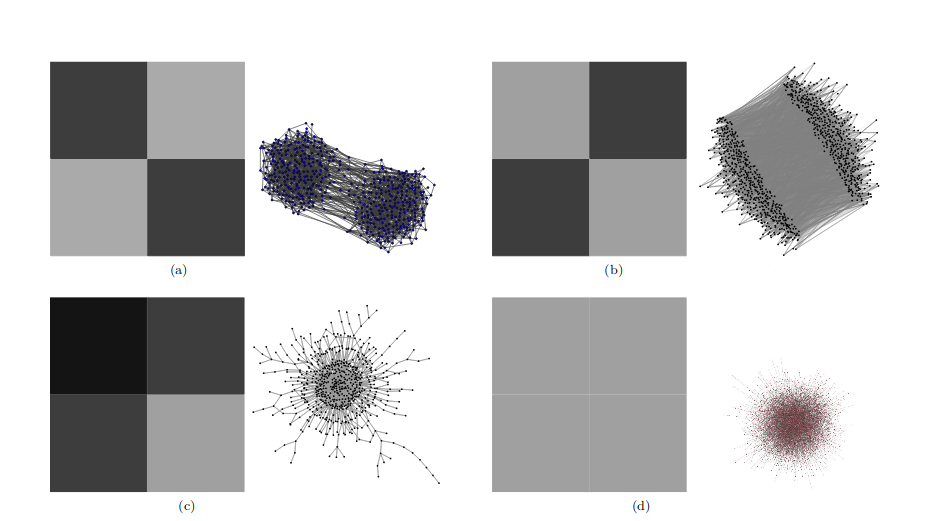
\includegraphics[width=0.5\textwidth]{Figures/structures.png}
	\caption{Stochastic Block model for different networks structures. (a) assortative. (b) dissortative. (c) core-periphery. (d) Erdos Renyi random graph.}
	\label{fig:SBM}
\end{figure}

A common definition of a community is that it is densely connected subgraph \cite{userguide}. We can find these subgraphs by optimizing an objective function, such as modularity function. It measures the difference in the number of edges between the given network and the network with the same number of nodes but randomly connected. In this approach, we try to maximize the density of connections inside a group by focusing more on assortative\footnote{Networks where nodes tend to connect with other nodes of a similar degree. Edges are more likely inside blocks than out of them.} group structures. 

Another type of networks is the bipartite network that has two disjoint sets of nodes. The edges exist only between nodes from different sets. Networks of this class can appear in real-world data, such as users-movies preference, collaboration network for scientists and papers, etc. Application of density-based approach requires to first project bipartite network to one of its partitions and then find communities in that projection. With this, some information is lost. On the other hand, the method that is directly applicable to bipartite networks is Stochastic Block model, from which the models considered in this paper are derived. \\

Stochastic block model (SBM) is based on connection probabilities between nodes. It is a generative model which includes existence of communities. Parameters that describe SBM for network G with N nodes are:

\begin{itemize}
	\item k: number of groups
	\item group assignment vector, g: $g_i \in\{1,2..k\}$, gives the group index of node $i$.
	\item SBM matrix, $p_{k \times k}$, whose elements $p_{ij}$ are the probabilities that edges between groups $g_i$ and $g_j$ exist.
\end{itemize}

Note that nodes within one group have the same connection probabilities.

SBM can generate and describe different types of network structures. Figure \ref{fig:SBM} \cite{userguide} shows how the model matrix corresponds to resulting networks with two communities. First, for the assortative network (\ref{fig:SBM} a), diagonal elements of the matrix have higher probabilities. This indicates dense connections inside the group, just like in classic community structures. In disassortative structure, (\ref{fig:SBM} b), more connections exist between two partitions than inside them, i.e. off-diagonal elements have higher probabilities. Bipartite networks can be represented like this. 

Figure (\ref{fig:SBM} c) shows how the model represents core-periphery networks. Nodes of one block (core) are well connected with itself and with other partition (periphery). From the last case, we can note that SBM with one group is the Erdos Renyi random graph (\ref{fig:SBM} d) because all probabilities inside and between groups are equal.

The benefit of this model is that we can generate many networks with similar group structure. The model can fit real data, which results in finding network communities. For the given network $G$ and number of groups $k$, the best nodes partition $g$ is found by maximizing the likelihood function. Beside inferring communities, SBM has application in prediction of missing links. This simply formulated model has many variants, motivated by specific properties of real data. For example, for networks which are degree heterogeneous, there is degree corrected SBM. In some social networks, users can belong to more than one group, and this can be modelled with mixed membership SBM. Other extensions include application to bipartite, weighted network, hierarchical model, etc. Also, several algorithms for optimization of likelihood function are proposed. The overview of these versions and methods are given in \cite{comparison}. In this paper, we will focus on Single and Mixed Membership SBM applied on bipartite networks.  